% !TeX root = ../relatorio-estagio.tex

\newpage
\section{Como \textit{Blockchain} é aplicado no mercado?}
\label{sec:blockchain_where}

No mercado existe uma grande variedade de implementações de \textit{blockchain}. Algumas implementações são aplicadas como bases de dados, sendo que outras são aplicadas como criptomoedas.

\subsection{Criptomoedas}

Criptomoedas são a forma mais popular de usar \textit{blockchain}. Existe um grande número de criptomoedas, porém baseiam-se num conceito base que foi evoluindo. Devido à evolução da ideia, criptomoedas podem-se separar em 3 gerações: ouro digital, contratos inteligentes e escalabilidade.

\subsubsection{\textit{Bitcoin}: Ouro Digital}

\begin{wrapfigure}{r}{2cm}
    
\includegraphics[width=2cm]{images/bitcoin.png}
    \caption{Logótipo do Bitcoin}
    \label{fig:bitcoin-logo}
\end{wrapfigure}

A primeira geração de criptomoedas é a aplicação de \textit{blockchain} para fins monetários, sendo o maior exemplo desta aplicação a criptomoeda \textit{Bitcoin} (\cref{fig:bitcoin-logo}).

``\textit{Bitcoin é uma criptomoeda descentralizada, sendo um dinheiro eletrónico para transações ponto-a-ponto. O primeiro artigo descrevendo uma implementação do Bitcoin foi criado em 2008 sendo apresentado no começo de 2009 a lista de discussão \textit{The Cryptography Mailing} por um programador ou grupo de programadores sob o pseudónimo Satoshi Nakamoto. Bitcoin é considerada a primeira moeda digital mundial descentralizada, constituindo um sistema económico alternativo, e responsável pelo ressurgimento do sistema bancário livre.}'' \cite{bitcoin_wiki}

\subsubsection{\textit{Ethereum}: Contratos Inteligentes}
\begin{wrapfigure}{r}{2cm}
    
\includegraphics[width=2cm]{images/ethereum.png}
    \caption{Logótipo do Ethereum}
    \label{fig:ethereum-logo}
\end{wrapfigure}

\textit{Ethereum} (\cref{fig:ethereum-logo}) é uma criptomoeda conceptualizada em 2013, inicializada em 2015 por Vitalik Buterin. Esta tem a especificidade de ter capacidade de executar contratos inteligentes e é a segunda cropitomoeda mais valorizada, estando atrás de \textit{Bitcoin}, no que toca a valor de mercado. \cite{ethereum_wiki}

Um contrato inteligente é um protocolo de computador auto executável criado com a popularização das criptomoedas. Contratos inteligentes são feitos para facilitar e reforçar a negociação ou desempenho de um contrato, proporcionando confiança em transações \textit{online}. Contratos inteligentes permitem que pessoas desconhecidas façam negócios de confiança entre si, pela Internet, sem a necessidade de intermédio de uma autoridade central.

\textit{Ethereum} também começou a implementação do seu \textit{upgrade}, chamado de \textit{Ethereum 2.0}, que inclui  técnologias como \acrfull{pos} e \textit{sharding}, que serão analisada em mais detalhe nas subsecções \ref{concenso} e \ref{sharding} respectivamente. 

\subsubsection{\textit{IOTA}: Escalabilidade}

\begin{wrapfigure}{r}{2cm}
    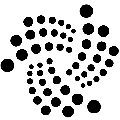
\includegraphics[width=2cm]{images/iota.png}
    \caption{Logótipo do IOTA}
    \label{fig:iota-logo}
\end{wrapfigure}

Publicada em 2016 por Serguei Popov e com o propósito de resolver o problema de baixo número de transações por segundo, \cite{iota_wiki} , \textit{IOTA}  (\cref{fig:iota-logo}) baseia se na ideia de \textit{Tangle}, isto é, em vez de usar uma \textit{blockchain} com uma única linha de blocos usa grafos acíclicos dirigidos.

Nesta rede não existem mineiros, a verificação de cada transição é feita
pelos dois nós anteriores. \cite{directed_acyclic_graph} Explicando de uma forma mais visual, pode se verificar na \cref{fig:linevsdag} que numa \textit{blockchain} normal, são adicionados blocos um a um sendo que 51\% da rede tem de estar em concordância resultando numa velocidade constante. No caso da \textit{IOTA} a velocidade estala com o número de blocos na rede já que blocos podem ser verificados em paralelo.


Para se alcançar consenso existe uma entidade central da fundação \textit{IOTA} que faz transições sem valor para verificar se os nós são legítimos.

\textit{IOTA} tem a desvantagem de ser centralizada pelo facto de ter
coordenadores que são entidades confiadas e centralizadas.

\begin{figure}[!ht]
    \centering
    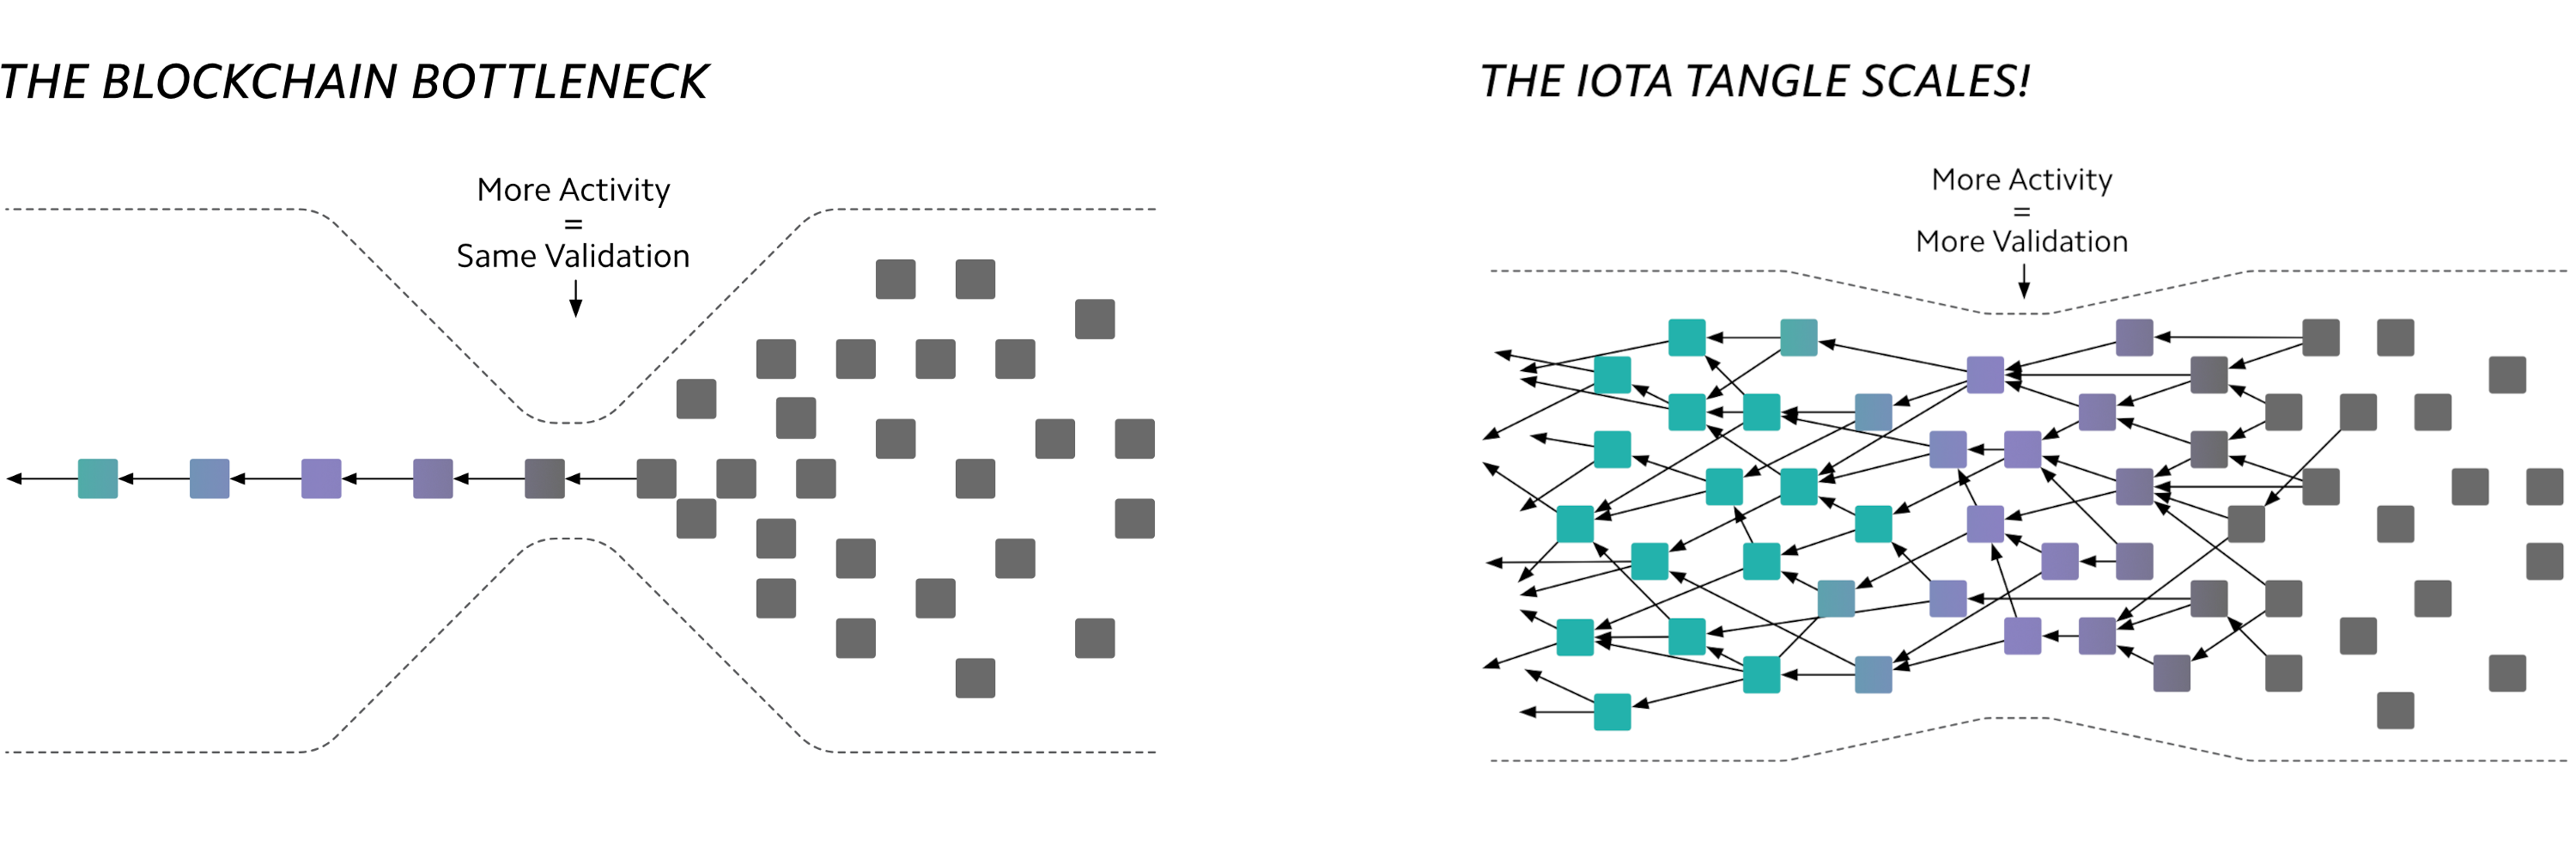
\includegraphics[width=\textwidth]{images/linevsdag.png}
    \caption{Uma \textit{Blockchain} comum comparada com o \textit{Tangle} do \textit{IOTA} (editada) \cite{iota_wiki}}
    \label{fig:linevsdag}
\end{figure}

\newpage
\subsection{Consensos}
\label{concenso}

\say{\textit{Um problema fundamental em sistemas de processamento distribuído é alcançar a confiança geral do sistema com a existência de processos defeituosos. Ademais, isso, normalmente, requer que processos concordem que algum dado ou valor seja necessário durante uma computação. Exemplos de aplicações de consenso distribuído incluem confirmar ou não uma transação para uma base de dados indefinida e concordar em relação à identidade de um líder.}}
 \cite{consensus_wiki}

Noutras palavras \textit{concensus} ou consenso na área da computação é o processo de confirmar que existe uma percentagem mínima de aplicações na rede que concordam com uma certa informação.

Existem vários algoritmos que podem fazer esse trabalho sendo que os de seguida apresentados parecem ser os mais utilizados:

\begin{itemize}
  \item
  \gls{pow} - é um sistema que cria um problema computacional
  cuja resolução tem um elevado custo de processamento mas é fácil de verificar. Como exemplo de implementação desta teoria refira-se a heurística de \textit{Fiat-Shamir} \cite{fiat-shamir_heuristic_wiki} 
  e o \textit{hashcash} que é o algoritmo usado pelo \textit{Bitcoin}. \cite{hashcash_wiki} É se chamado aqueles que fazem as verificações de mineiros. \cite{miners}

\item
  \gls{pos} - é um sistema que, em vez de criar um problema
  computacional para se verificar uma transição, coloca em causa o
  dinheiro daqueles que querem verificar. Se alguém quiser manipular de
  forma maliciosa uma transação terá, não só de ter 51\% do dinheiro que
  existe numa \textit{blockchain}, como também deve estar pronto a arriscar perder
  o dinheiro e fazer o seu valor descer, desencorajando assim ataques por causa do alto risco.
  Outra vantagem reside no facto de não ser preciso dispositivos de alto poder computacional para efetuar verificações. \cite{proof-of-stake}
  
\end{itemize}

\subsection{\textit{Sharding}}
\label{sharding}
\textit{Sharding} é o conceito de subdividir uma base de dados para que se melhore a sua escalabilidade. Isto é, quanto maior for o número de utilizadores na rede, melhor deve ser a divisão de trabalho. No contexto de \textit{blockchain}, quanto maior o número de utilizadores, maior o número de transições por segundo. \cite{sharding_geeks}

A implementação de \textit{sharding} é mais comum em bases de dados e criptomoedas com entidades confiadas pela rede como \textit{IOTA}, sendo a presença de \textit{sharding}  em criptomoedas públicas e descentralizadas sem elementos confiados ou favorecidos muito menos comum.

\subsection{Framework e Protocolos}

Também foram encontradas várias aplicações e \textit{frameworks} que podiam ser utilizadas ou poderiam servir como inspiração para aplicar no projeto. Uma lista dessa aplicações/ \textit{frameworks} poderá ser vista na tabela \ref{table:frameworks}.

\begin{table}[h!]
  \centering
  \begin{tabularx}{\linewidth}{>{\hsize=.3\hsize}lX}
    \multicolumn{1}{c}{\textbf{Nome}} & 
    \multicolumn{1}{c}{\textbf{Descrição}}
    \tabularnewline \tabularnewline 
    \textit{Hyperledger}&
    Uma \textit{pool} de projetos, apoiada pela \textit{Linux foundation}, relacionados com \textit{blockchain}. \cite{hyperledger}
    \tabularnewline \midrule
    \textit{BigchainDB}&
    Base de dados em \textit{blockchain}. Construída com base em \textit{consensus} de um líder. \cite{bigchaindb}
    \tabularnewline \midrule
    \acrfull{ipfs}&
    ``\textit{Sistema de Ficheiros Interplanetário é um protocolo e uma rede projetada para criar um armazenamento associativo ponto-a-ponto endereçável ao conteúdo de armazenamento e compartimentação, de hipermédia, num sistema de ficheiros distribuído.}'' \cite{ipfs_wiki}
    \tabularnewline \midrule
    \textit{Ethereum Casper}&
    \textit{Casper} é o protocolo que os pesquisadores de \textit{Ethereum} estão a estudar e a desenvolver para implementar \acrshort{pos} e \textit{sharding} em \textit{Ethereum}. \cite{ethereum_casper}
    \tabularnewline \midrule
    \end{tabularx}
  \caption{\textit{Frameworks} e Protocolos}
  \label{table:frameworks}
\end{table}
